% ----------------------------------------------------------
% Subseção Consciência
% ----------------------------------------------------------
\subsection{Consciência}
Um momento lógico pode ser formado por uma divisão (primeiro momento) ou por subdivisões lógicas (demais momentos).
	\begin{figure}[H]
	\caption{Intervalo lógico}
	\label{fig:consciousness_logical_moments}
	\centering
	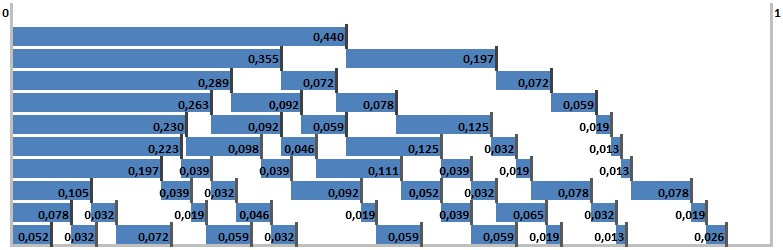
\includegraphics[scale=.7]{sections/images/consciousness_logical_moments.jpg}
	\floatfoot{Exemplo de um intervalo lógico com dez momentos lógicos.}%\footnotemark}
	\end{figure}
	%\footnotetext{Fonte: note}

A consciência são os momentos lógicos de uma expansão representados em suas unidades.
	\begin{figure}[H]
	\caption{Intervalo lógico consciente}
	\label{fig:consciousness}
	\centering
	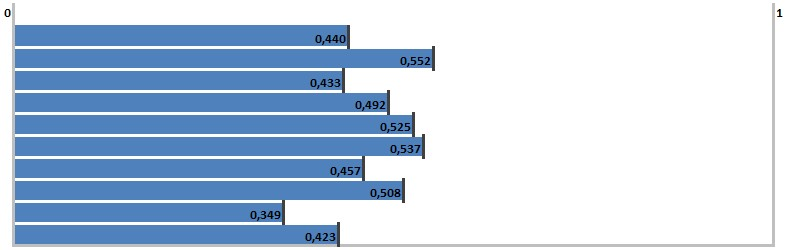
\includegraphics[scale=.7]{sections/images/consciousness.jpg}
	\floatfoot{Exemplo de um intervalo lógico consciente com dez unidades de momentos lógicos.}%\footnotemark}
	\end{figure}
	%\footnotetext{Fonte: note}

Pode ser observado na Tabela \ref{tab:10000_all} que a probabilidade de 99,99\% das amostras (Amostras do Range), que aumentam em quantidade a medida que crescem os momentos lógicos, tendem a estar cada vez mais ao centro do intervalo lógico, sendo que essa centralização tende ao infinito.
	\begin{figure}[H]
	\caption{Centralização de 99,99\% das amostras}
	\label{fig:centering_of_99_range}
	\centering
	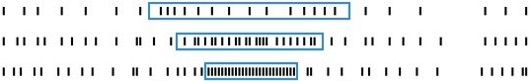
\includegraphics[scale=1]{sections/images/centering_of_99_range.jpg}
	\floatfoot{Tendência de centralização do range de 99,99\% das amostras.}%\footnotemark}
	\end{figure}
	%\footnotetext{Fonte: note}

A consciência tende à representação de um histograma da distribuição normal. Todos os aspectos listados abaixo são inerentes a abstração lógica chamada consciência.

\subsubsection{Infinito}
Um dos aspectos mais importantes que a negação do nada traz (negação de si), é o infinito, ou seja, em qualquer intervalo lógico cabe o infinito novamente. A lógica primordial que iniciou todo o intervalo lógico é a mesma encontrada em seus intervalos subsequentes. Isso fundamenta como uma lógica de alto nível como a subconsciência humana explica a lógica primordial, uma vez que não é preciso voltar ao primeiro momento lógico do intervalo para deduzi-lo, pois esse fenômeno é onipresente em todo o intervalo.

\subsubsection{Ondas}
Probabilisticamente a distribuição de novas amostras de uma população tendem a concentrar mais amostras sentido a mediana da população com frequências de amostras cada vez maiores neste sentido. Porém, a distribuição dessas amostras com frequências de crescimento uniformes é infinitesimal se comparado às possibilidades randômicas desse crescimento. Assim, a tendência de crescimento dessas frequências sentido a mediana somadas a baixíssima probabilidade (infinitesimal) desse crescimento ser uniforme, conduz a frequências no padrão de ondas.
	\begin{figure}[H]
	\caption{Padrão de onda}
	\label{fig:consciousness_waves}
	\centering
	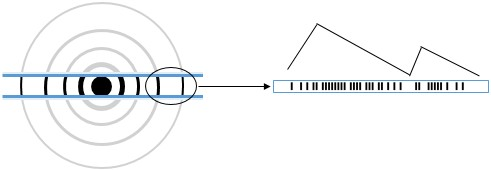
\includegraphics[scale=1]{sections/images/consciousness_waves.jpg}
	\floatfoot{Padrão de onda inferido pela tendência dessa distribuição com frequências maiores sentido a mediana da população e a baixíssima probabilidade de crescimento uniforme dessas frequências.}%\footnotemark}
	\end{figure}
	%\footnotetext{Fonte: note}

A junção de duas ondas além de eliminar suas discrepâncias, faz com que a primeira onda da união fique maior e a segunda onda acabe por deixar de existir a se tornar parte da primeira, que tem seu pico mais próximo da mediana. Probabilisticamente uma onda não morre, apenas une-se com outras ondas mais centrais a ela.
	\begin{figure}[H]
	\caption{Unificação de ondas}
	\label{fig:consciousness_uniform_wave}
	\centering
	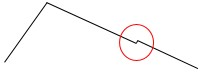
\includegraphics[scale=1]{sections/images/consciousness_uniform_wave.jpg}
	\floatfoot{Ondas sendo unificadas para exemplificar o crescimento amostral uniforme.}%\footnotemark}
	\end{figure}
	%\footnotetext{Fonte: note}

\subsubsubsection{Entrelaçamento e subconsciente}
As amostras que mais se parecem em termos de frequências e distribuição são as amostras que fazem parte da mesma onda. Elas são frequências opostas não sobrepostas que se completam.

Probabilisticamente as duas partes complementares de uma onda estarão a uma distância aproximadamente iguais, equidistante da mediana, porém essa não é uma regra e as partes complementares de uma onda podem estar em distâncias diferentes da mediana. O fenômeno da paridade das partes de uma onda tem o nome de entrelaçamento de ondas.

Essas ondas formam subconsciências de uma consciência maior. A consciência é única para todo o intervalo, é a lógica do intervalo, enquanto formam subconsciências ou sub-lógicas, como pequenas ondas de uma onda maior. Assim, uma mudança na onda maior (consciência) também é uma mudança na onda menor (subconsciência), mudança essa que é induzida pelas subconsciências indiretamente, análogo ao comprimir gás em um cilindro, onde ao adicionar uma nova molécula de gás no cilindro parcialmente cheio, mais próximas ou apertas as moléculas dentro dele estarão. O contrário também é verdadeiro, uma nova amostra em uma subconsciência que por esta é observada diretamente é também uma mudança da consciência e vai ser induzida por outras subconsciências indiretamente.
	\begin{figure}[H]
	\caption{Subconsciência}
	\label{fig:consciousness_subconscious}
	\centering
	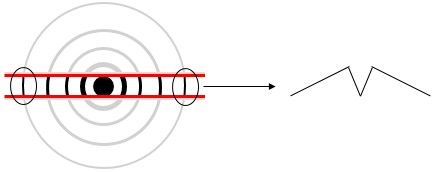
\includegraphics[scale=1]{sections/images/consciousness_subconscious.jpg}
	\floatfoot{O padrão de ondas forma subconsciências semelhantes ao padrão criado pela consciência (histograma de distribuição normal) como visto na Figura \ref{fig:statisticsbyjim_central_limit_theorem} ou na Figura \ref{fig:trend_chart_of_normal_distribution}.}%\footnotemark}
	\end{figure}
	%\footnotetext{Fonte: note}

\subsubsubsection{Salto}
O salto é uma reordenação feita pelo entrelaçamento de ondas a medida que as amostras do entrelaçamento deixam de ser equivalentes com a adição de novas amostras em seus lados.

Na Figura \ref{fig:consciousness_space_subconscious_observation_jump} é observado os entrelaçamento de ondas (representadas por colunas do histograma na vertical). A reordenação feita pelo entrelaçamento provoca um salto nas coordenadas (X, Y e Z) conforme subseção do Espaço.
	\begin{figure}[H]
	\caption{Reordenação subconsciente - Salto}
	\label{fig:consciousness_space_subconscious_observation_jump}
	\centering
	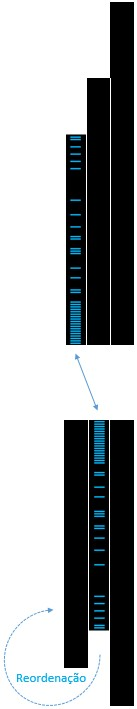
\includegraphics[scale=.6]{sections/images/consciousness_space_subconscious_observation_jump.jpg}
	\floatfoot{Salto provocado pela não equivalência do entrelaçamento com a adição de novas amostras.}%\footnotemark}
	\end{figure}
	%\footnotetext{Fonte: note}

A tendência probabilística é que, por exemplo, o elétron que saltou de sua orbita de origem retorne à esta conforme mais amostras são adicionadas ao entrelaçamento desse átomo, estabelecendo a normalidade probabilística.

\subsubsection{Tempo}
O tempo é a adição de novos momento lógicos entre momentos existentes à medida que prossegue a negação de si da lógica. Essas mudanças são acumulativas e a medida que aumentam o número desses momentos lógicos, menos relevante cada novo momento será dentro do intervalo consciente. Um em cem é mais relevante do que um em mil. 
	\begin{figure}[H]
	\caption{Tempo}
	\label{fig:consciousness_time}
	\centering
	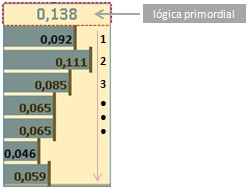
\includegraphics[scale=.8]{sections/images/consciousness_time.jpg}
	\floatfoot{Progressão do tempo conforme os momentos lógicos avançam.}%\footnotemark}
	\end{figure}
	%\footnotetext{Fonte: note}

Outro fator importante a observar do tempo é que, probabilisticamente, subconsciências mais próximas da mediana da população terão uma adição maior de novas amostras em seus intervalos, o que são observados diretamente por essas subconsciências. Por outro lado, subconsciências distantes da mediana da população terão uma adição menor de amostras em seus intervalos e sujeitam-se a um número maior de mudança induzidas indiretamente. Esse fenômeno de observação temporal proporcionado pela consciência e subconsciências evita o paradoxo dos gêmeos \cite{brasilescola_paradoxo_gemeos}.

Na seção Expansão lógica foi apresentado que a lógica é uma sequência de negações de si no tempo zero, ou seja, em nenhum momento entre suas negações a lógica passa a SER, garantindo a premissa primordial da constante lógica, NÃO SER. Assim, a lógica é uma sequência infinita e simultânea, uma constante. Logo, o tempo é apenas uma grandeza da consciência oriunda da ordenação dessa sequência lógica, não da sequência propriamente. A simultaneidade dessa sequência torna a lógica uma constante com todas as suas infinitas possibilidades, sendo esse universo uma delas. 

Cada universo tem uma ordem diferente em sua sequência e é essa ordem que dá origem à grandeza que chamamos de tempo. É essa ordem do universo ou consciência que vai dar a noção do que acontece antes ou depois, ou seja, o passado, o presente e o futuro. 

Na experiência do tempo conduzida pela consciência a ordenação da sequência é a essência dessa grandeza e, portanto, mais relevante do que sua origem que é de natureza simultânea.

\subsubsection{Espaço}
As ondas da consciência exibidas em forma de histograma, onde as partes das ondas que se completam são colocados lado a lodo é exibida na Figura \ref{fig:consciousness_space_waves}. A formação desse histograma é proveniente do entrelaçamento de ondas.
	\begin{figure}[H]
	\caption{Histograma proveniente do entrelaçamento de ondas}
	\label{fig:consciousness_space_waves}
	\centering
	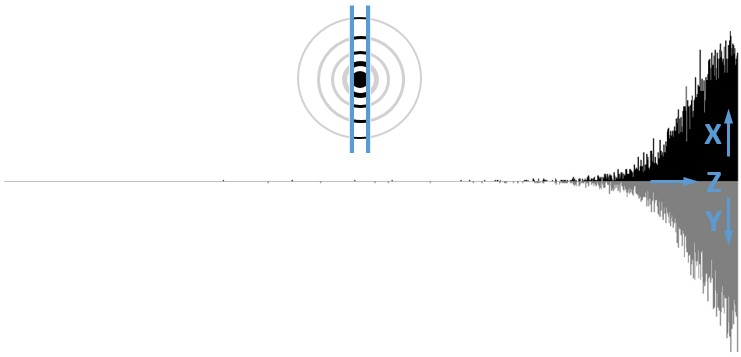
\includegraphics[scale=.7]{sections/images/consciousness_space_waves.jpg}
	\floatfoot{Exemplo do padrão de ondas obtido pelo algoritmo Logic\_WavePattern. \footnotemark}
	\end{figure}
	\footnotetext{O algoritmo Logic\_WavePattern pode ser visto no Apêndice \ref{app:algoritmos}.}

Ao representar as grandezas espaciais do gráfico da Figura \ref{fig:consciousness_space_waves} em um gráfico de distribuição 3D e distribuir seus pontos de extremidade (desprezando seus volumes e possíveis pontos internos), obtém-se algo parecido com uma espiral (como redemoinhos no ar ou na água) mesmo em volumes muito pequenos de dados (poucos momentos lógicos), conforme Figuras \ref{fig:consciousness_space_3DScatter15000-10} e \ref{fig:consciousness_space_3DScatter_200000-2}. Os pontos se movem em formato de espiral, aproximadamente, uma vez que as coordenadas X, Y e Z aumentam à medida que novas amostras são adicionadas na população.
	\begin{figure}[H]
	\centering
		\begin{subfigure}[H]{0.47\linewidth}
		\centering
		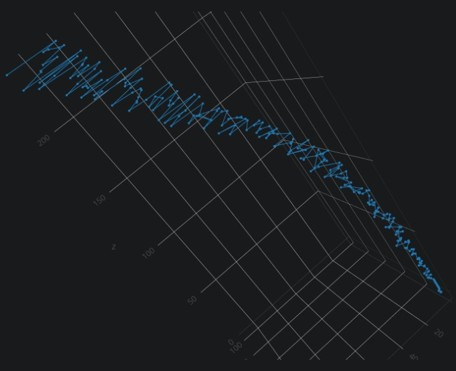
\includegraphics[width=.96\linewidth]{sections/images/consciousness_space_3DScatter15000-10.jpg}
		\caption{15.000 amostras ou momentos}
		\label{fig:consciousness_space_3DScatter15000-10}
		\end{subfigure}
	\hfill
		\begin{subfigure}[H]{0.47\linewidth}
		\centering
		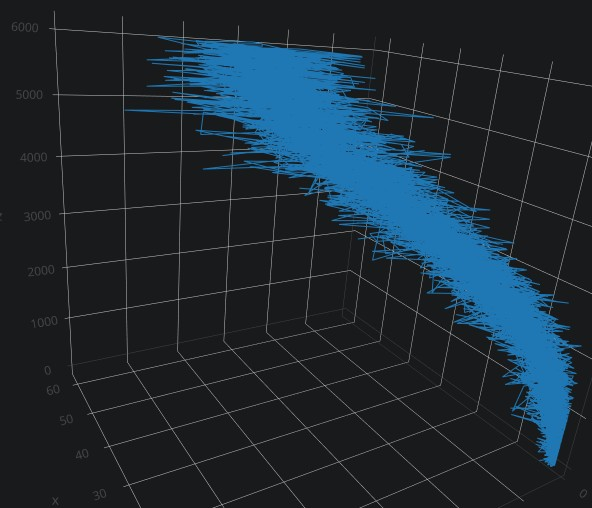
\includegraphics[width=.9\linewidth]{sections/images/consciousness_space_3DScatter_200000-2.jpg}
		\caption{200.000 amostras ou momentos}
		\label{fig:consciousness_space_3DScatter_200000-2}
		\end{subfigure}%
	\caption{Gráfico de dispersão 3D gerado com os pontos da Figura \ref{fig:consciousness_space_waves}}
	\floatfoot{O histograma no padrão de ondas e os dados para gerar o gráfico de dispersão 3D podem ser obtidos com a execução do algoritimo Logic\_WavePattern. \protect\footnotemark}
	\end{figure}
	\footnotetext{O algoritmo Logic\_WavePattern pode ser visto no Apêndice \ref{app:algoritmos} e os gráficos de dispersão 3D podem ser acessados em: \url{https://chart-studio.plot.ly/create/?fid=ren.stuchi:5&fid=ren.stuchi:4} e \url{https://chart-studio.plot.ly/create/?fid=ren.stuchi:7&fid=ren.stuchi:6}}

\subsubsubsection{Comprimento de onda - Intervalo}
A observação de outras subconsciências (sub-lógicas) depende do range de ondas (comprimento de ondas) que uma subconsciência é capaz de observar e esse range, que por sua vez depende do comprimento de ondas que a própria subconsciência é constituída. Todos os possíveis intervalos que se correspondem em X e Y encontram-se simultaneamente formando ondas em diferentes níveis. Dentre todas as possibilidades de intervalos ou comprimento de ondas permitidos por uma população, o observador está um deles ou em um range deles. Alguns exemplos de comprimentos de ondas podem ser observados na Figura \ref{fig:consciousness_space_subconsciousness_examples}.
	\begin{figure}[H]
	\caption{Diferentes comprimentos de ondas - intervalos}
	\label{fig:consciousness_space_subconsciousness_examples}
	\centering
	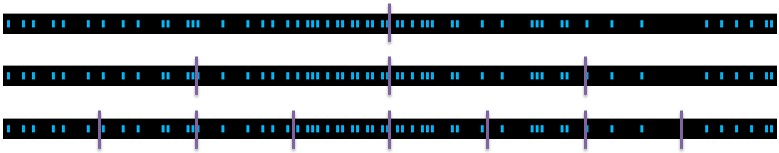
\includegraphics[scale=.5]{sections/images/consciousness_space_subconsciousness_examples.jpg}
	\floatfoot{Exemplo de diferentes comprimentos de ondas.}%\footnotemark}
	\end{figure}
	%\footnotetext{Fonte: note}
	
Em ranges de muitos momentos lógicos pode-se ver o agrupamento de grandes objetos (subconsciências), sendo o maior deles representado pela cor azul claro e os menores e mais distantes pela cor azul escuro ou roxo, conforme Figura \ref{fig:consciousness_space_subconsciousness}. Esse agrupamento pode representar, por exemplo, o centro do universo, então o centro de uma galáxia, estrelas, planetas e objetos menores e mais distantes.
	\begin{figure}[H]
	\caption{Abstração espacial das subconsciências - grandes agrupamentos}
	\label{fig:consciousness_space_subconsciousness}
	\centering
	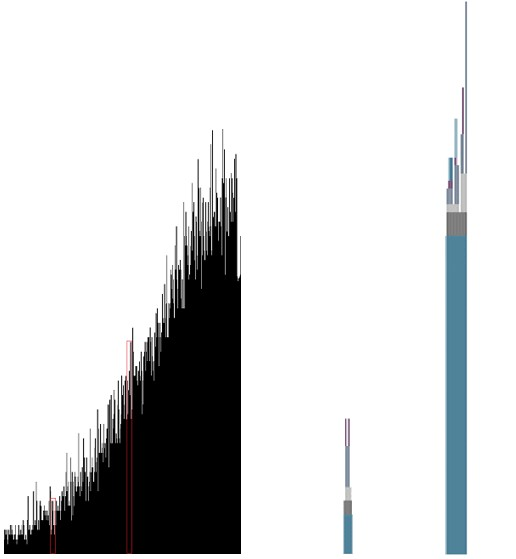
\includegraphics[scale=.45]{sections/images/consciousness_space_subconsciousness.jpg}
	\floatfoot{Caracteristicas da ondas formadoras da subconsciência de grandes objetos.}%\footnotemark}
	\end{figure}
	%\footnotetext{Fonte: note}

Em ranges com uma quantidade menor de momentos lógicos pode-se ver o agrupamento de pequenos objetos (subconsciências). Quanto menores os agrupamentos menos divisões esses agrupamentos têm (cores) e mais estreitos e compridos eles são, conforme Figura \ref{fig:consciousness_space_subconsciousness_min}. Esse agrupamento pode representar, por exemplo, o átomo que são muito pequenos, se apresentam em enormes quantidades e as partículas que orbitam seu núcleo (elétrons) ficam bem mais distantes dele.
	\begin{figure}[H]
	\caption{Abstração espacial das subconsciências - pequenos agrupamentos}
	\label{fig:consciousness_space_subconsciousness_min}
	\centering
	
\includegraphics[scale=.7]{sections/images/consciousness_space_subconsciousness_min.jpg}
	\floatfoot{Caracteristicas da ondas formadoras da subconsciência de pequenas partículas.}%\footnotemark}
	\end{figure}
	%\footnotetext{Fonte: note}}
	
As cores dos agrupamentos indicam a relação entre conjuntos e subconjuntos. Subconjuntos nascem de conjuntos ou outros subconjuntos e essa relação paterna filial é permanente. Conjuntos e subconjuntos também podem se dividir no mesmo nível, a depender do entrelaçamento das amostras.

\subsubsubsection{Amplitude de onda - Volume}
Da parte inicial da Figura \ref{fig:consciousness_space_volume} originam-se duas observações. A primeira que a altura das colunas do histograma (amplitude) é diretamente relacionada a quantidade de amostras ou momentos lógicos do intervalo (comprimento). A segunda observação é que a densidade de distribuição das amostras de uma coluna do histograma é inalterada. Graficamente é o mesmo que colocar o intervalo (comprimento de onda) na vertical.

O volume dobra a cada um terço de crescimento das amostras ou momentos lógicos de um agrupamento, aproximadamente. Ao imaginar uma esfera com o diâmetro equivalente à amplitude dessa onda unificada, ou seja, com o comprimento dessa onda referente à todo o objeto, a parte mais facilmente observável é onde está a maior concentração de amostras desse intervalo, que é sentido à mediana da população, probabilisticamente, conforme visto na Figura \ref{fig:consciousness_space_volume}.
\begin{figure}[H]
	\caption{Amostras vs volume}
	\label{fig:consciousness_space_volume}
	\centering
	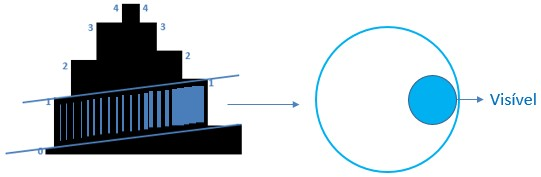
\includegraphics[scale=1]{sections/images/consciousness_space_volume.jpg}
	\floatfoot{O volume em três dimensões dobra a cada um terço de crescimento das amostras, aproximadamente.}%\footnotemark}
	\end{figure}
	%\footnotetext{Fonte: note}}

\subsubsubsection{Espiral}
O padrão de espiral observado na Figura \ref{fig:consciousness_space_spiral} é fundamentado pelo entrelaçamento de ondas, a base para formação do espaço, e o padrão probabilístico descrito pelo teorema central do limite, onde as amostras de uma população tendem sentido à mediana. O padrão de espiral observado não invalida outros possíveis movimentos no espaço. Muitas vezes não é possível observar o padrão de espiral imediatamente nos movimentos de subconsciências, porém parece que este padrão está por traz de muitos destes movimentos, pois ao pegar os movimentos humanos como exemplo tem-se os ciclos predominantes de ir e voltar para casa, ir e voltar ao trabalho, acordar e dormir, ou seja, os hábitos parecem movimentos em círculos, movimentos espirais.
	\begin{figure}[H]
	\caption{Padrão do movimento em espiral}
	\label{fig:consciousness_space_spiral}
	\centering
	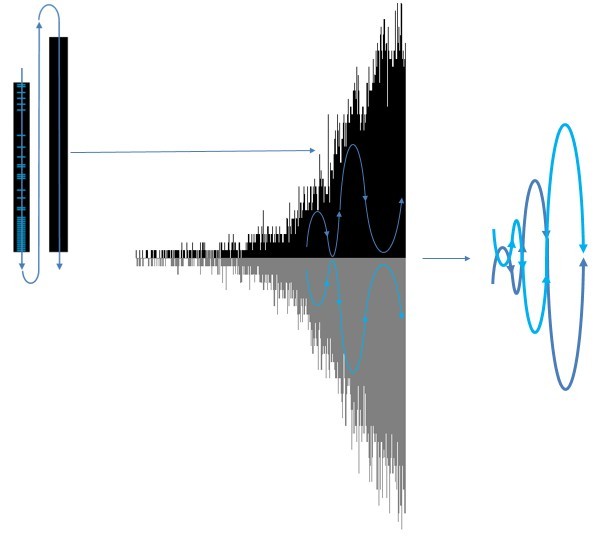
\includegraphics[scale=.65]{sections/images/consciousness_space_spiral.jpg}
	\floatfoot{Detalhes do movimento em espiral dos subconjuntos de amostras.}%\footnotemark}
	\end{figure}
	%\footnotetext{Fonte: note}}

Como as coordenadas X, Y e Z de cada subconjunto tendem a aumentar, a disposição dessas em um sistema tridimensional de coordenadas vai seguir uma referência diagonal entre esses três eixos, conforme Figura \ref{fig:consciousness_space_spiral_reference_line}.

Na Figura \ref{fig:consciousness_space_spiral_reference_line} pode ser observado também os pontos X1 e X2. Esses pontos foram espelhados nas coordenadas X e Z para facilitar a observação de que as amostras de um intervalo tende a aumentar em todas as coordenadas. Assim, por mais que X2 esteja representando a média mínima probabilística do objeto A para esse determinado ponto Z, ela é ainda maior que X1, a média máxima probabilística do objeto A para um ponto Z anterior.
	\begin{figure}[H]
	\caption{Sistema tridimensional de coordenadas}
	\label{fig:consciousness_space_spiral_reference_line}
	\centering
	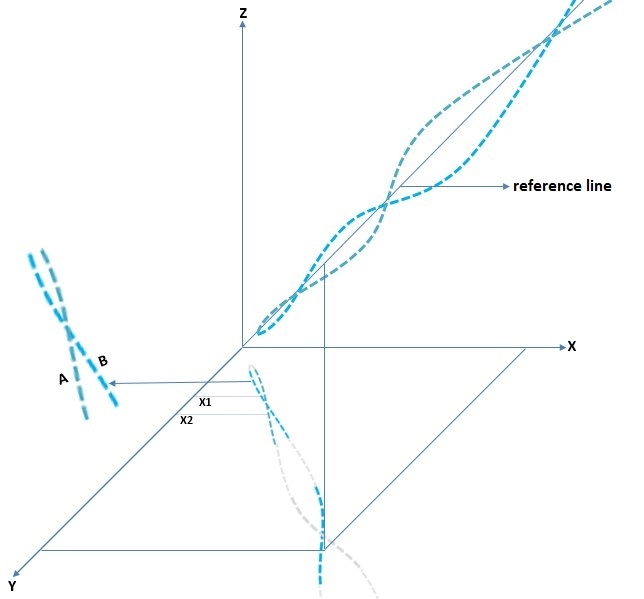
\includegraphics[scale=.7]{sections/images/consciousness_space_spiral_reference_line.jpg}
	\floatfoot{Linha de referência para distribuição de uma população em um plano tridimensional.}%\footnotemark}
	\end{figure}
	%\footnotetext{Fonte: note}}

Os subconjuntos capazes de sobreviver por ciclos espirais (os subconjuntos mais próximos da base, como o subconjunto 1, são mais resilientes) estarão com suas coordenadas X e Y entres os pontos médios máximos e médios mínimos probabilísticos para determinado range em Z, conforme Figura \ref{fig:consciousness_space_spiral_undulation}. Assim, se o objeto B está em seu ponto médio máximo probabilístico, onde subconjunto 1 do bloco 1 estejam como a maior parte das amostras dentro do range de alta densidade, por exemplo. Ao seguir o ciclo esse objeto tenderá a ir para o ponto médio mínimo probabilístico, onde subconjunto 1 do bloco 1 estejam como a maior parte das amostras dentro do range de baixa densidade.
	\begin{figure}[H]
	\caption{Média mínima e média máxima probabilísticas}
	\label{fig:consciousness_space_spiral_undulation}
	\centering
	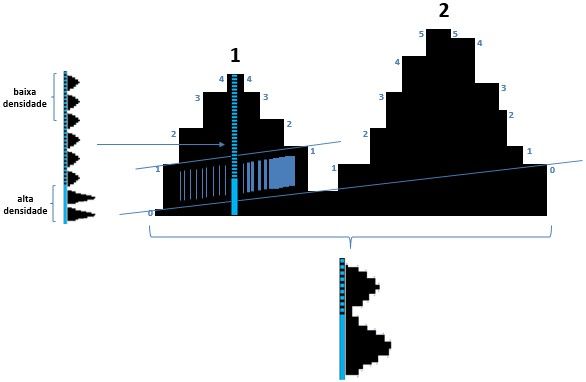
\includegraphics[scale=.6]{sections/images/consciousness_space_spiral_undulation.jpg}
	\floatfoot{Média mínima e média máxima probabilísticas das coordenadas em relação à linha de referência.}%\footnotemark}
	\end{figure}
	%\footnotetext{Fonte: note}}

Na Figura \ref{fig:consciousness_space_spiral_direction} é exibida a orientação da parte facilmente visível de um objeto juntamente com o espaço que completa a formação deste objeto. A parte facilmente observável probabilisticamente encabeça o movimento, conforme visto na Figura \ref{fig:consciousness_space_spiral_undulation} (na barra azul mais à direita do histograma no bloco 1 subconjunto 1), uma vez que as maiores densidades de amostras estão nas barras do histograma sentido à mediana, podendo as altas densidades estarem mais na parte superior ou inferior de um subconjunto, como o subconjunto 1.
	\begin{figure}[H]
	\caption{Orientação do movimento em espiral}
	\label{fig:consciousness_space_spiral_direction}
	\centering
	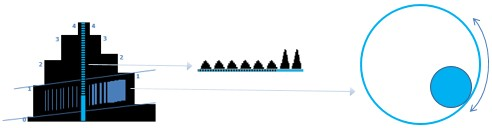
\includegraphics[scale=1]{sections/images/consciousness_space_spiral_direction.jpg}
	\floatfoot{Orientação do movimento em espiral da parte visível de um objeto em relação ao espaço que o completa.}%\footnotemark}
	\end{figure}
	%\footnotetext{Fonte: note}}

A adição de novas amostras à uma população cria novos subconjuntos e isso acontece em frequências muito altas em agrupamentos menores como os átomos ou ainda menores. Isso faz com que novos subconjuntos sejam criados antes (menor frequência) e depois (maior frequência sentido à mediana) de um subconjunto especifico. É o mesmo que dizer que átomos serão formados antes e depois de um átomo especifico. E é isso que faz com que um objeto se movimente à frente enquanto fica cada vez mais distante da mediana da população.

Cada agrupamento tem sua própria linha de referência. Assim como dentro de um metro existem os centímetros, milímetros etc., dentro de um agrupamento existem outros agrupamentos.
	\begin{figure}[H]
	\caption{Intervalos e linhas de referências}
	\label{fig:consciousness_space_spiral_underlines}
	\centering
	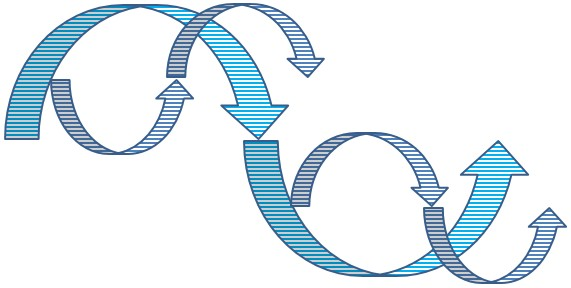
\includegraphics[scale=.5]{sections/images/consciousness_space_spiral_underlines.jpg}
	\floatfoot{Espirais em diferentes intervalos e suas linhas de referências.}%\footnotemark}
	\end{figure}
	%\footnotetext{Fonte: note}}

O acumulo de amostras em um intervalo de uma coordenada provoca uma elevação dessa coordenada. Um exemplo desses picos são os satélites, onde esses picos os colocam em orbita afastada da terra. A manutenção dessa orbita é sustentada pela manutenção constante desse pico de intervalo, o que promove uma aceleração no tempo. Como visto na subseção de Tempo, as amostras mais próximas da mediana, onde são mais frequentes esses intervalos com um número maior de amostras (pico), sofrem uma adição maior de amostras diretamente em relação aos intervalos longe da mediana que acabam induzindo essas mudanças indiretamente. 

\subsubsection{Forças fundamentais}
A força gravitacional, a força eletromagnética e a força nuclear correspondem às forças fundamentais da natureza e essas forças também são provenientes do entrelaçamento de ondas, como o espaço. As forças fundamentais não são forças propriamente, mas sim aspectos probabilísticos (distribuição normal) e do entrelaçamento de ondas principalmente.

\subsubsubsection{Força gravitacional}
O entrelaçamento ondas é o aspecto que coordena as mudanças nas coordenadas espaciais junto com a adição de novos momentos lógicos sentido a mediana da população. As mudanças dessas coordenadas provocam iterações que podem ser vistas nas Figuras \ref{fig:consciousness_space_3DScatter15000-10} e \ref{fig:consciousness_space_3DScatter_200000-2} da subseção de Espaço e na Figura \ref{fig:consciousness_dark_matter_dark_energy_wave} que mostra probabilisticamente onde está a maior concentração de momentos lógicos de um intervalo consciente ou subconsciente, devido a estes momentos serem mais intensos sentido a mediana. Estes aspectos são chamadas de gravidade.

\subsubsubsection{Força eletromagnética}
A força eletromagnética é uma especificação do aspecto gravitacional que depende da aproximação espacial (redução de diferenças nos eixos X, Y e Z) e do entrelaçamento de ondas.

Quando um objeto se aproxima de outro, seus pares de ondas provenientes do entrelaçamento de ondas ficam cada vez mais parecidos, eixos X e Y. Essa proximidade faz com que as partes das ondas de um objeto se pareça muito com as partes das ondas do outro objeto, o que pode fazer com que o entrelaçamento de ondas encontre pares mais ideais nesse outro objeto e vice-versa.  

As linhas azuis da Figura \ref{fig:consciousness_electromaagnetic_force} mostra onde é mais frequente a troca dos pares de ondas pelo entrelaçamento de ondas, ou seja, onde se tem a maior probabilidade das ondas serem parecidas. Por isso os imãs tentam se virar para se conectar quando estão face a face com o mesmo polo. As linhas cinza mostram as conexões que ocorrem em número bem menor. 
	\begin{figure}[H]
	\caption{Força eletromagnética}
	\label{fig:consciousness_electromaagnetic_force}
	\centering
	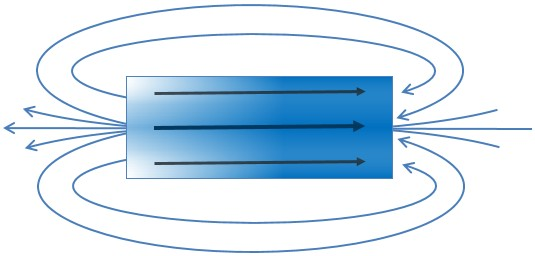
\includegraphics[scale=.6]{sections/images/consciousness_electromaagnetic_force.jpg}
	\floatfoot{Aumento das possibilidades de entrelaçamento de ondas devida a aproximação e o menor número de momentos lógicos das menores partículas. }%\footnotemark}
	\end{figure}
	%\footnotetext{Fonte: note}

Com a troca de significativos pares de ondas entre os objetos faz-se a mixagem do posicionamento dos eixos X, Y e Z entre esses objetos ocorrendo a aproximação deles no espaço. 

Quanto menor a partícula (elétron ou partículas menores), conforme Figura \ref{fig:consciousness_space_subconsciousness_min}, mais fácil o entrelaçamento ocorre. Provavelmente muitos objetos não tenham alta capacidade de entrelaçamento devido aos seus elétrons ou partículas menores serem formadas por muitos momentos lógicos (barras do histograma mais largas ou mais compridas), ou seja, quanto maior a quantidade de momentos dessas partículas menores as chances de entrelaçamento.

Probabilisticamente as partículas mais parecidas estão nas regiões mais próximas (linhas azuis do Figura \ref{fig:consciousness_electromaagnetic_force}) devido ao crescimento do número de amostras sentido a mediana da população, porém isso não é uma regra e os polos podem se inverter, ou seja, ter mais ligações com a região de menor probabilidade (isso não quer dizer que houve formação de antimatéria nessa região, as partículas ainda tendem a concentrar mais momentos lógicos sentido à mediana da população). No entanto, a probabilidade tende a corrigir esses polos conforme novos momentos vão sendo adicionadas nesse intervalo.

\subsubsubsection{força nuclear}
As forças nucleares forte e fraca representam as maiores concentrações de momentos lógicos por intervalo populacional. Esses picos podem ser vistos na Figura \ref{fig:consciousness_space_subconsciousness_min} e eles não param de crescer à medida que novos momentos lógicos são adicionados nestes intervalos. Estes momentos ou amostras tendem a estarem cada vez mais juntos dentro do intervalo formando picos cada vez mais altos.

\subsubsection{Matéria escura e energia escura}
Quanto maior o número de amostras e mais próximas elas estão da mediana, mais elas farão parte dos 99,99\% e ainda mais amostras também estarão nos 0,01\%, conforme a Tabela \ref{tab:10000_all}. Logo, a energia escura não é uma energia propriamente, mas sim um aspecto probabilístico. 
	\begin{figure}[H]
	\caption{Aspecto probabilístico da energia escura}
	\label{fig:consciousness_dark_matter_dark_energy}
	\centering
	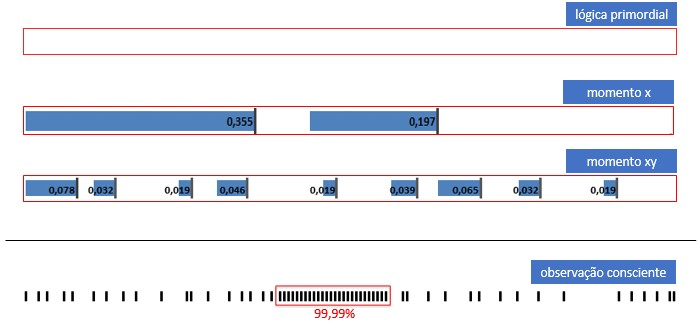
\includegraphics[scale=.9]{sections/images/consciousness_dark_matter_dark_energy.jpg}
	\floatfoot{A energia escura não é uma energia propriamente, mas sim um aspecto probabilístico.}%\footnotemark}
	\end{figure}
	%\footnotetext{Fonte: note}

Já a matéria escura, como pode ser visto na Figura \ref{fig:consciousness_dark_matter_dark_energy_wave} mostra probabilisticamente onde está a maior concentração das amostras de um intervalo, tornando mais fácil a visualização por outras subconsciências, uma vez também que o volume dobra a cada um terço do crescimento das colunas do histograma, aproximadamente, conforme dito na seção do Espaço. Assim, uma grande área do intervalo de um agrupamento pode conter amostras dispersas que se tornam mais difíceis de observar. O aspecto descrito acima e demostrado pela Figura \ref{fig:consciousness_dark_matter_dark_energy_wave} é aplicável a qualquer intervalo de um agrupamento (Figuras \ref{fig:consciousness_space_subconsciousness} e \ref{fig:consciousness_space_subconsciousness_min}).
	\begin{figure}[H]
	\caption{Analogia da matéria escura}
	\label{fig:consciousness_dark_matter_dark_energy_wave}
	\centering
	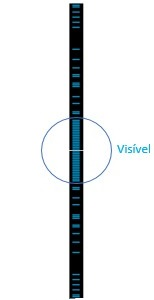
\includegraphics[scale=.75]{sections/images/consciousness_dark_matter_dark_energy_wave.jpg}
	\floatfoot{Parte do volume é facilmente observado por outras subconsciências.}%\footnotemark}
	\end{figure}
	%\footnotetext{Fonte: note}

\subsubsection{Antimatéria}
Independente do intervalo observado, sua maior concentração de amostras tende a estar sentido da mediana, o que é o sentido provável conforme teorema central do limite. Essas amostras também podem estar com sua concentração no sentido oposto à mediana, porém com uma ocorrência probabilística cada vez menos conforme as amostras aumentam. Na Figura \ref{fig:consciousness_concentration_of_opposite_samples} é exibido dois intervalos idênticos com suas amostras com concentrações opostas.
	\begin{figure}[H]
	\caption{Parte de um intervalo idêntico com suas concentrações de amostras opostas}
	\label{fig:consciousness_concentration_of_opposite_samples}
	\centering
	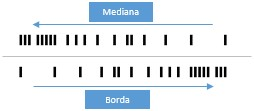
\includegraphics[scale=1]{sections/images/consciousness_concentration_of_opposite_samples.jpg}
	\floatfoot{Parte de um intervalo idêntico distribuídos de formas opostas.}%\footnotemark}
	\end{figure}
	%\footnotetext{Fonte: note}

O merge ou soma dos intervalos opostos da Figura \ref{fig:consciousness_concentration_of_opposite_samples} os tornaria um intervalo simétrico, ou seja, não estaria em nenhum dos sentidos.
Na Figura \ref{fig:consciousness_concentration_of_opposite_samples_within_range} é exibido um intervalo consciente completo com suas concentrações de amostras sentido à mediana e outro idêntico, mas com suas concentrações sentido às bordas do intervalo.
	\begin{figure}[H]
	\caption{Intervalos conscientes com suas concentrações de amostras opostas}
	\label{fig:consciousness_concentration_of_opposite_samples_within_range}
	\centering
	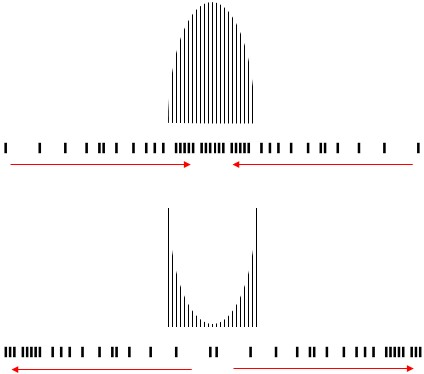
\includegraphics[scale=.8]{sections/images/consciousness_concentration_of_opposite_samples_within_range.jpg}
	\floatfoot{Intervalos conscientes completos e idênticos distribuídos de formas opostas.}%\footnotemark}
	\end{figure}
	%\footnotetext{Fonte: note}


\subsubsection{Buraco negro}
O buraco negro é uma concentração muito alta de amostras, formada por grandes agrupamentos subconscientes, Figura \ref{fig:consciousness_space_subconsciousness}.
Esses grandes agrupamentos ocupam grandes volumes de espaço devido a quantidade de amostras. 

Os grandes volumes são encontrados na base dos grandes agrupamentos, conforme as cores azul claro e cinza da Figura \ref{fig:consciousness_black_hole}.
	\begin{figure}[H]
	\caption{Buracos negros}
	\label{fig:consciousness_black_hole}
	\centering
	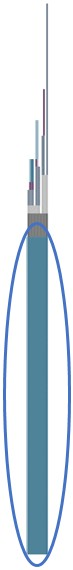
\includegraphics[scale=.6]{sections/images/consciousness_black_hole.jpg}
	\floatfoot{Grandes volumes são encontrados na base dos grandes agrupamentos.}%\footnotemark}
	\end{figure}
	%\footnotetext{Fonte: note}